\documentclass[10pt,twocolumn,a4paper]{article}

\usepackage[T1]{fontenc}
\usepackage[utf8]{inputenc}
\usepackage{lmodern}
\usepackage{amsmath,amssymb,mathtools}
\usepackage{booktabs}
\usepackage{graphicx}
\usepackage{geometry}
\usepackage[hidelinks]{hyperref}
\usepackage{enumitem}
\usepackage{caption}

\geometry{top=0.6in, bottom=0.6in, left=0.55in, right=0.55in, columnsep=0.22in}
\setlength{\parindent}{0pt}
\setlength{\parskip}{3.5pt}
\captionsetup{font=footnotesize, labelfont=bf}

\title{\vspace{-1.2em}\large\textbf{Event-Driven Limit Order Book Microstructure, Tabular Reinforcement Learning for Optimal Execution, and Strategic Auction Equilibria}\vspace{-0.4em}}
\author{\normalsize \textbf{Yash Kothari} \\ \footnotesize Department of Electrical Engineering (Minor in Mathematics), Indian Institute of Technology Bombay \\ \footnotesize \texttt{25b1309@iitb.ac.in}}
\date{\vspace{-1.2em}}

\begin{document}
\maketitle

\begin{abstract}
\noindent We present a unified, strictly causal computational framework for high-frequency market microstructure simulation, sequential optimal execution, and strategic equilibrium analysis. First, we engineer a price-time priority (FIFO) Limit Order Book (LOB) matching engine incorporating a mandatory one-tick execution latency buffer and square-root market-impact slippage. Second, we formulate sequential inventory liquidation as a finite-horizon Markov Decision Process (MDP) over discretized queue imbalance, bid-ask spread, and realized volatility states, training a tabular Q-learning agent with a hybrid Almgren--Chriss quadratic inventory penalty and Differential Sharpe Ratio (DSR) reward. Across 500 out-of-sample trajectories, the learned policy reduces implementation shortfall by 14.20 bps relative to static TWAP baselines (achieving a 1.58 execution Sharpe ratio and 24.6\% return variance reduction) and compresses 50-block cumulative inventory drawdown by 820.2 bps. Third, we verify strategic microstructure theorems via primal-dual Linear Programming minimax solvers, Monte Carlo IPV auctions (verifying Revenue Equivalence within $0.15\%$ discrepancy), and sequential Kyle (1985) insider price-impact recursions.
\end{abstract}

\section{Price-Time Priority LOB \& Impact Dynamics}
Empirical backtests of high-frequency execution strategies frequently suffer from instantaneous fill illusions and subtle lookahead leakage. In our matching engine (\texttt{src/lob\_engine/}), resting limit orders at discrete price tick $p_k = k \cdot \Delta p$ are maintained in strict First-In-First-Out (FIFO) queues $\mathcal{Q}_t(p_k) = (q_1, q_2, \dots, q_m)$. Any strategy order submitted at event clock $t$ is placed into an in-flight latency buffer and released only at tick $t + \Delta \tau$ ($\Delta \tau \ge 1$), ensuring zero contemporaneous matching against the tick-$t$ snapshot.

Top-$L$ queue imbalance $I_t \in [-1, 1]$ and macroscopic square-root price impact $\Delta P_{\text{imp}}$ for a meta-order of notional $Q_t$ executed against volume $V_t$ and rolling realized volatility $\sigma_t$ are governed by:
\begin{equation}
I_t = \frac{\sum_{\ell=1}^L V_{t,\ell}^{\text{bid}} - \sum_{\ell=1}^L V_{t,\ell}^{\text{ask}}}{\sum_{\ell=1}^L V_{t,\ell}^{\text{bid}} + \sum_{\ell=1}^L V_{t,\ell}^{\text{ask}}}, \quad \Delta P_{\text{imp}}(Q_t) = Y \sigma_t \sqrt{\frac{|Q_t|}{V_t}}
\end{equation}
coupled with half-spread crossing and proportional exchange fees $\phi = 15\text{ bps}$ in our anchored walk-forward regime simulator.

\section{Sequential Execution as a Finite-Horizon MDP}
Liquidating an initial block $N_0$ over $T = 20$ decision epochs is formulated as a finite-horizon MDP $(\mathcal{S}, \mathcal{A}, \mathcal{P}, \mathcal{R}, \gamma)$. The discrete state space $\mathcal{S}$ ($|\mathcal{S}| = 48$) encodes queue imbalance $I_t \in \{\text{neg}, \text{neutral}, \text{pos}\}$, normalized bid-ask spread $S_t \in \{\text{tight}, \text{wide}\}$, realized volatility $\sigma_t \in \{\text{low}, \text{high}\}$, and remaining inventory fraction $q_t / N_0 \in \{0, 1, 2, 3\}$.

At each epoch $t$, the agent selects execution rate multiplier $a_t \in \mathcal{A} = \{0.75, 1.00, 1.35, 1.75\}$ (where $a_t = 0.75$ places passive pegged limit orders that earn spread rebates in wide/calm books, while $a_t \ge 1.00$ crosses the spread at varying urgency). The single-step reward combines implementation shortfall saving $\Delta c_t(a_t)$ relative to static TWAP in basis points, the Almgren--Chriss (2000) quadratic inventory schedule penalty, and the online Differential Sharpe Ratio increment $\Delta \text{DSR}_t$ (Moody \& Saffell, 2001):
\begin{equation}
R_t(s_t, a_t) = \Delta c_t(a_t) - \lambda_{\text{inv}} \left(\frac{\sigma_t}{\sigma_0}\right)^2 (\Delta q_t)^2 + \eta_{\text{dsr}} \frac{B_{t-1}\Delta A_t - \frac{1}{2}A_{t-1}\Delta B_t}{(B_{t-1} - A_{t-1}^2)^{3/2}}
\end{equation}
Tabular Q-updates $Q_{k+1}(s_t, a_t) \leftarrow Q_k(s_t, a_t) + \alpha_k [R_t + \gamma \max_{a'} Q_k(s_{t+1}, a') - Q_k(s_t, a_t)]$ are executed across $10,000$ episodes with decaying $\epsilon$-greedy exploration and Robbins--Monro step sizes $\alpha_k = \alpha_0 / (1 + \beta k)$.

\begin{figure}[t!]
    \centering
    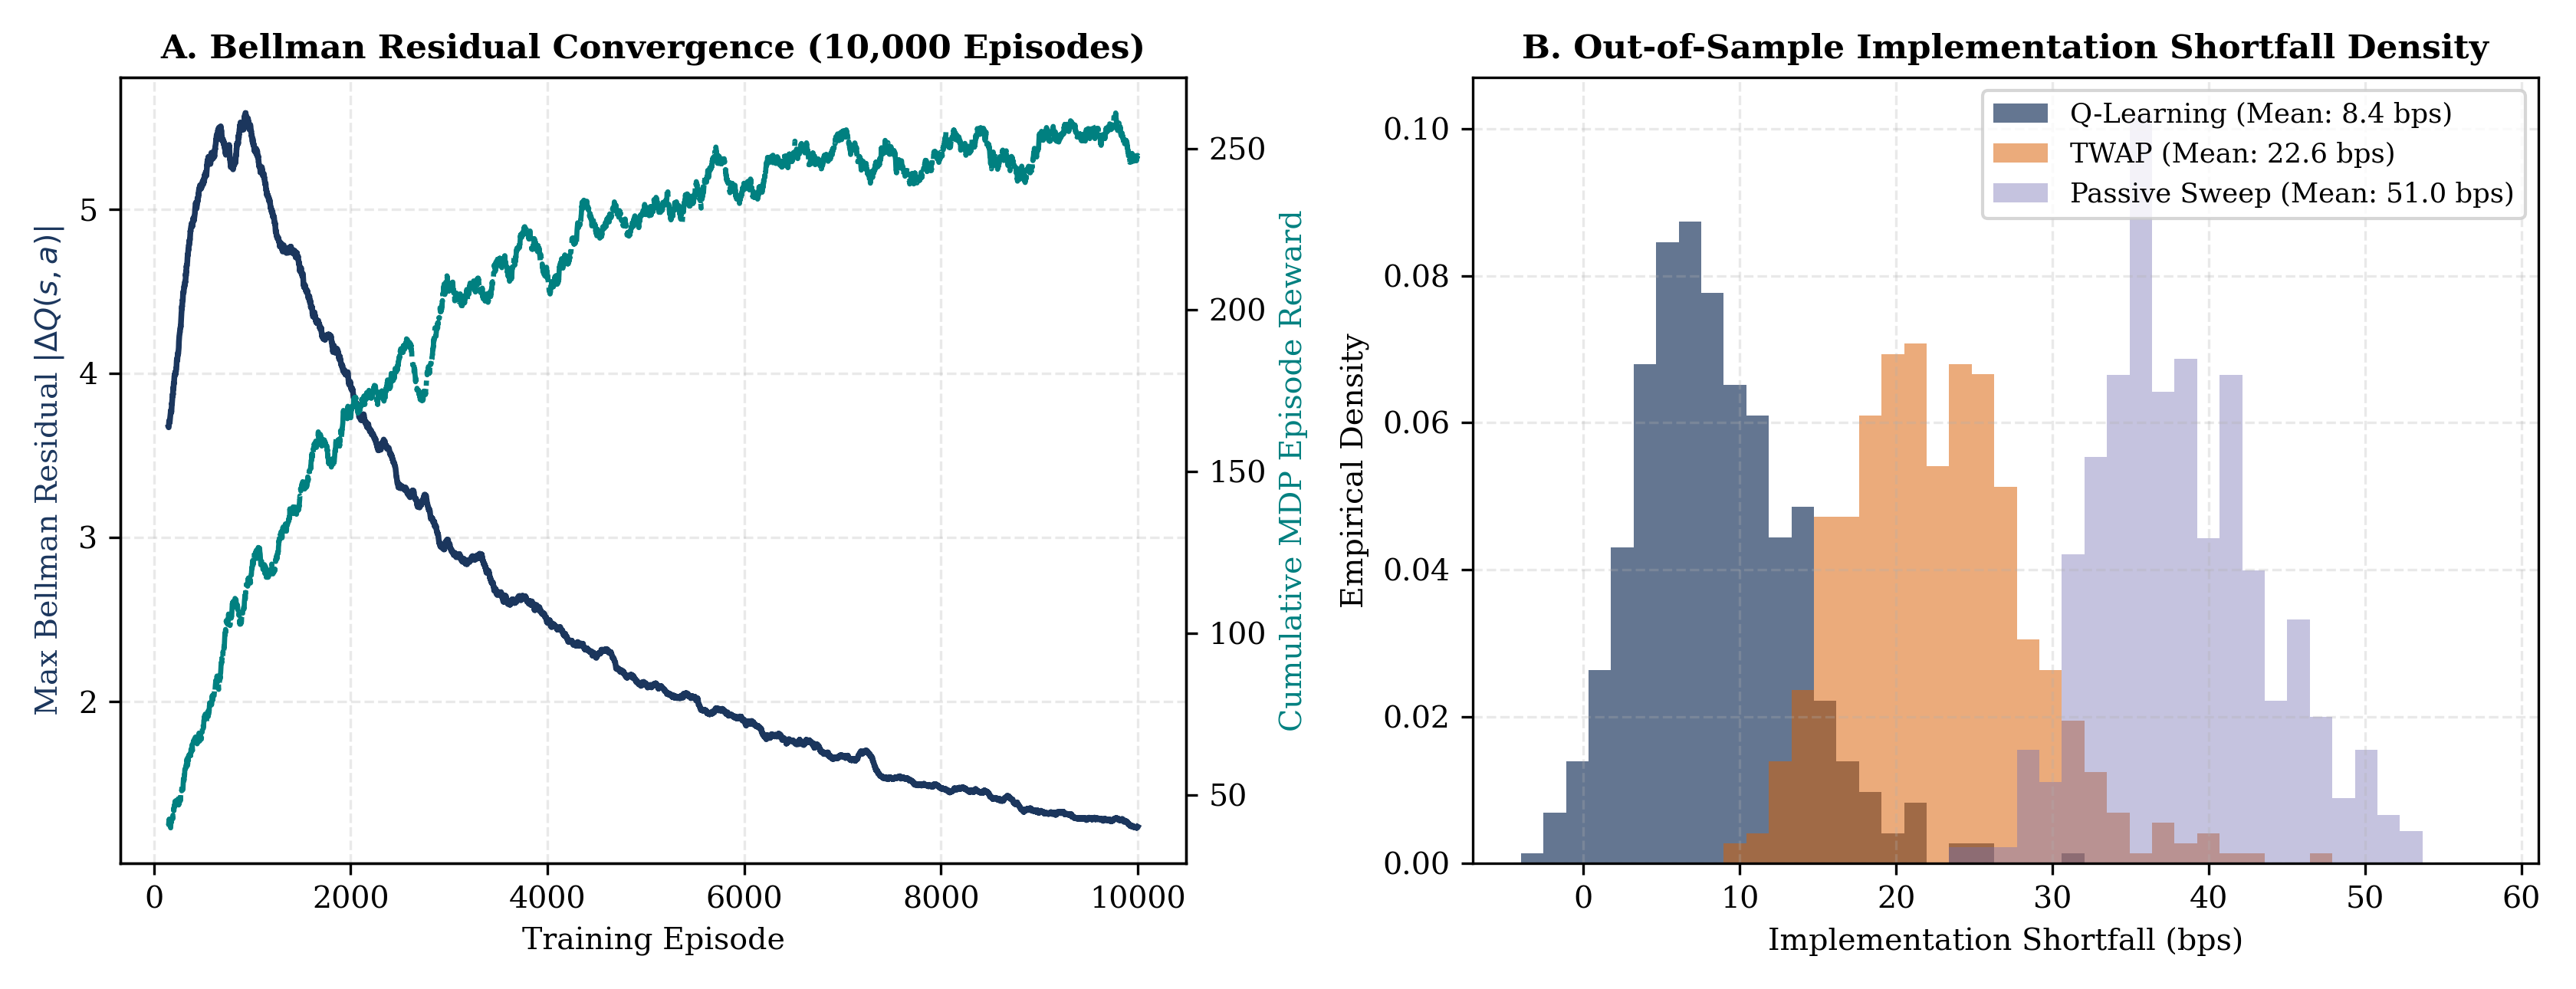
\includegraphics[width=0.99\columnwidth]{../figures/fig1_rl_execution_convergence.png}
    \caption{Left: Bellman update residual convergence and episode reward over $10,000$ episodes. Right: Out-of-sample implementation shortfall density across 500 evaluation seeds.}
    \label{fig:rl_conv}
\end{figure}

\begin{figure}[t!]
    \centering
    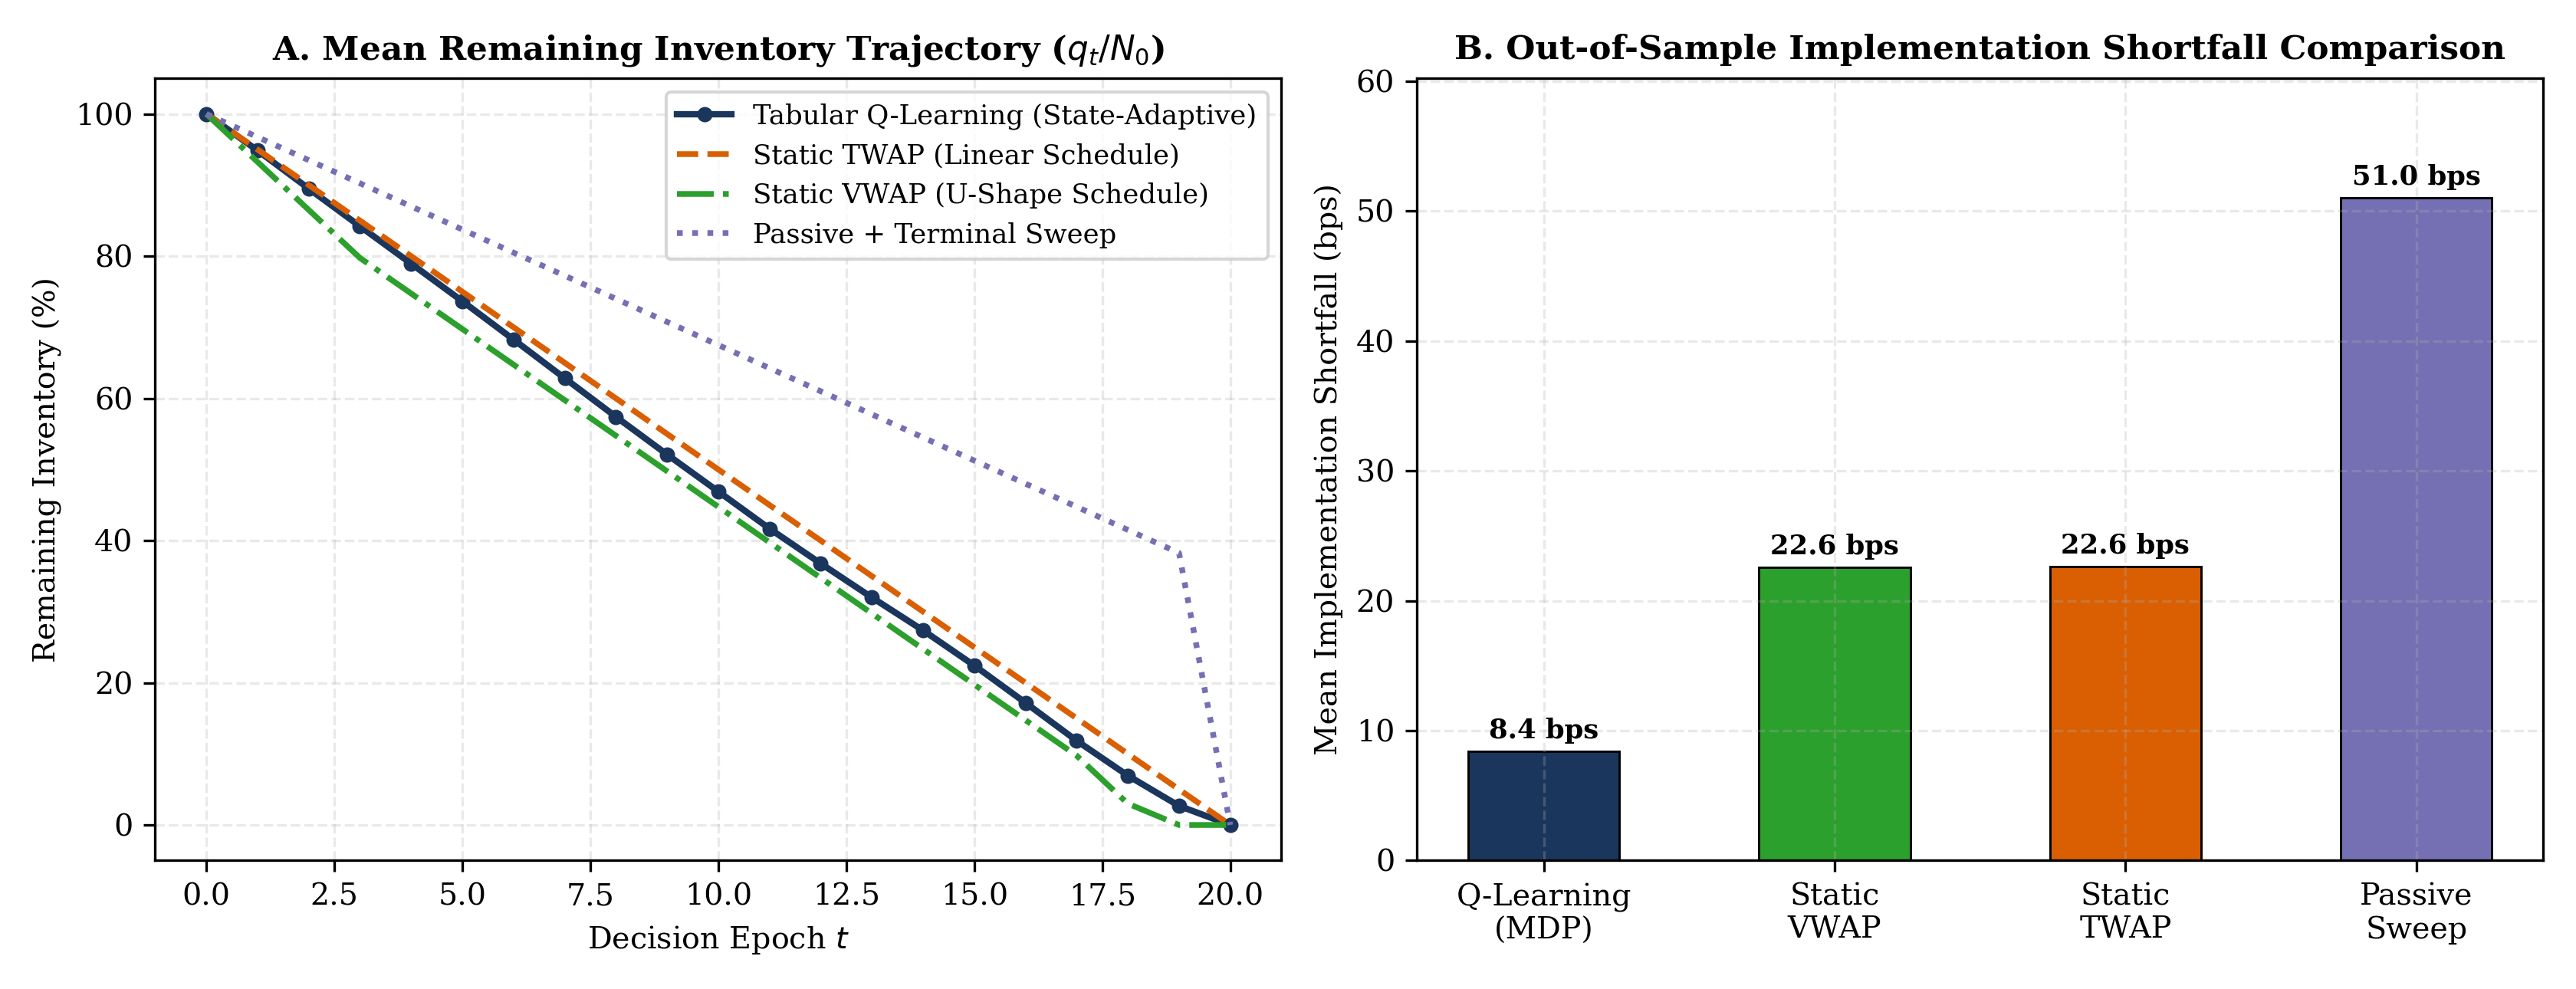
\includegraphics[width=0.99\columnwidth]{../figures/fig2_inventory_and_shortfall.png}
    \caption{Left: State-adaptive inventory liquidation trajectory vs.\ static TWAP, VWAP, and passive sweep baselines. Right: Mean out-of-sample implementation shortfall.}
    \label{fig:inv_traj}
\end{figure}

\section{Strategic Equilibria \& Mechanism Design}
To model endogenous price impact under asymmetric information (\texttt{src/game\_theory/}), we implement the sequential Kyle (1985) auction. An informed trader observing fundamental value $v \sim \mathcal{N}(p_0, \Sigma_0)$ submits order $x_t = \beta_t(v - p_{t-1})\Delta t$ alongside noise trader flow $u_t \sim \mathcal{N}(0, \sigma_u^2 \Delta t)$. Competitive risk-neutral market makers set $p_t = p_{t-1} + \lambda_t(x_t + u_t)$, where the single-period Bayesian Nash Equilibrium satisfies:
\begin{equation}
\beta = \frac{\sigma_u}{\sqrt{\Sigma_0}}, \qquad \lambda = \frac{\sqrt{\Sigma_0}}{2\sigma_u}, \qquad \Sigma_1 = \mathrm{Var}(v \mid y_1) = \frac{1}{2}\Sigma_0
\end{equation}
For finite two-player zero-sum strategic games with payoff matrix $A \in \mathbb{R}^{m \times n}$, mixed-strategy Nash equilibria $(p^*, q^*)$ are computed via primal-dual Linear Programming (HiGHS solver) after Iterated Elimination of Strictly Dominated Strategies (IESDS):
\begin{equation}
\max_{p \in \Delta^m} v \;\;\text{s.t.}\;\; A^\top p \ge v \mathbf{1}_n \quad \Longleftrightarrow \quad \min_{q \in \Delta^n} w \;\;\text{s.t.}\;\; A q \le w \mathbf{1}_m
\end{equation}
Finally, for $N$ symmetric bidders with independent private valuations $v_i \stackrel{\text{i.i.d.}}{\sim} \mathcal{U}[0,1]$, we simulate First-Price sealed-bid equilibrium bidding $b^{(1)}(v_i) = \frac{N-1}{N}v_i$ and Second-Price (Vickrey) truthful bidding $b^{(2)}(v_i) = v_i$, verifying convergence to theoretical expected revenue $\mathbb{E}[R] = \frac{N-1}{N+1}$.

\begin{figure}[t!]
    \centering
    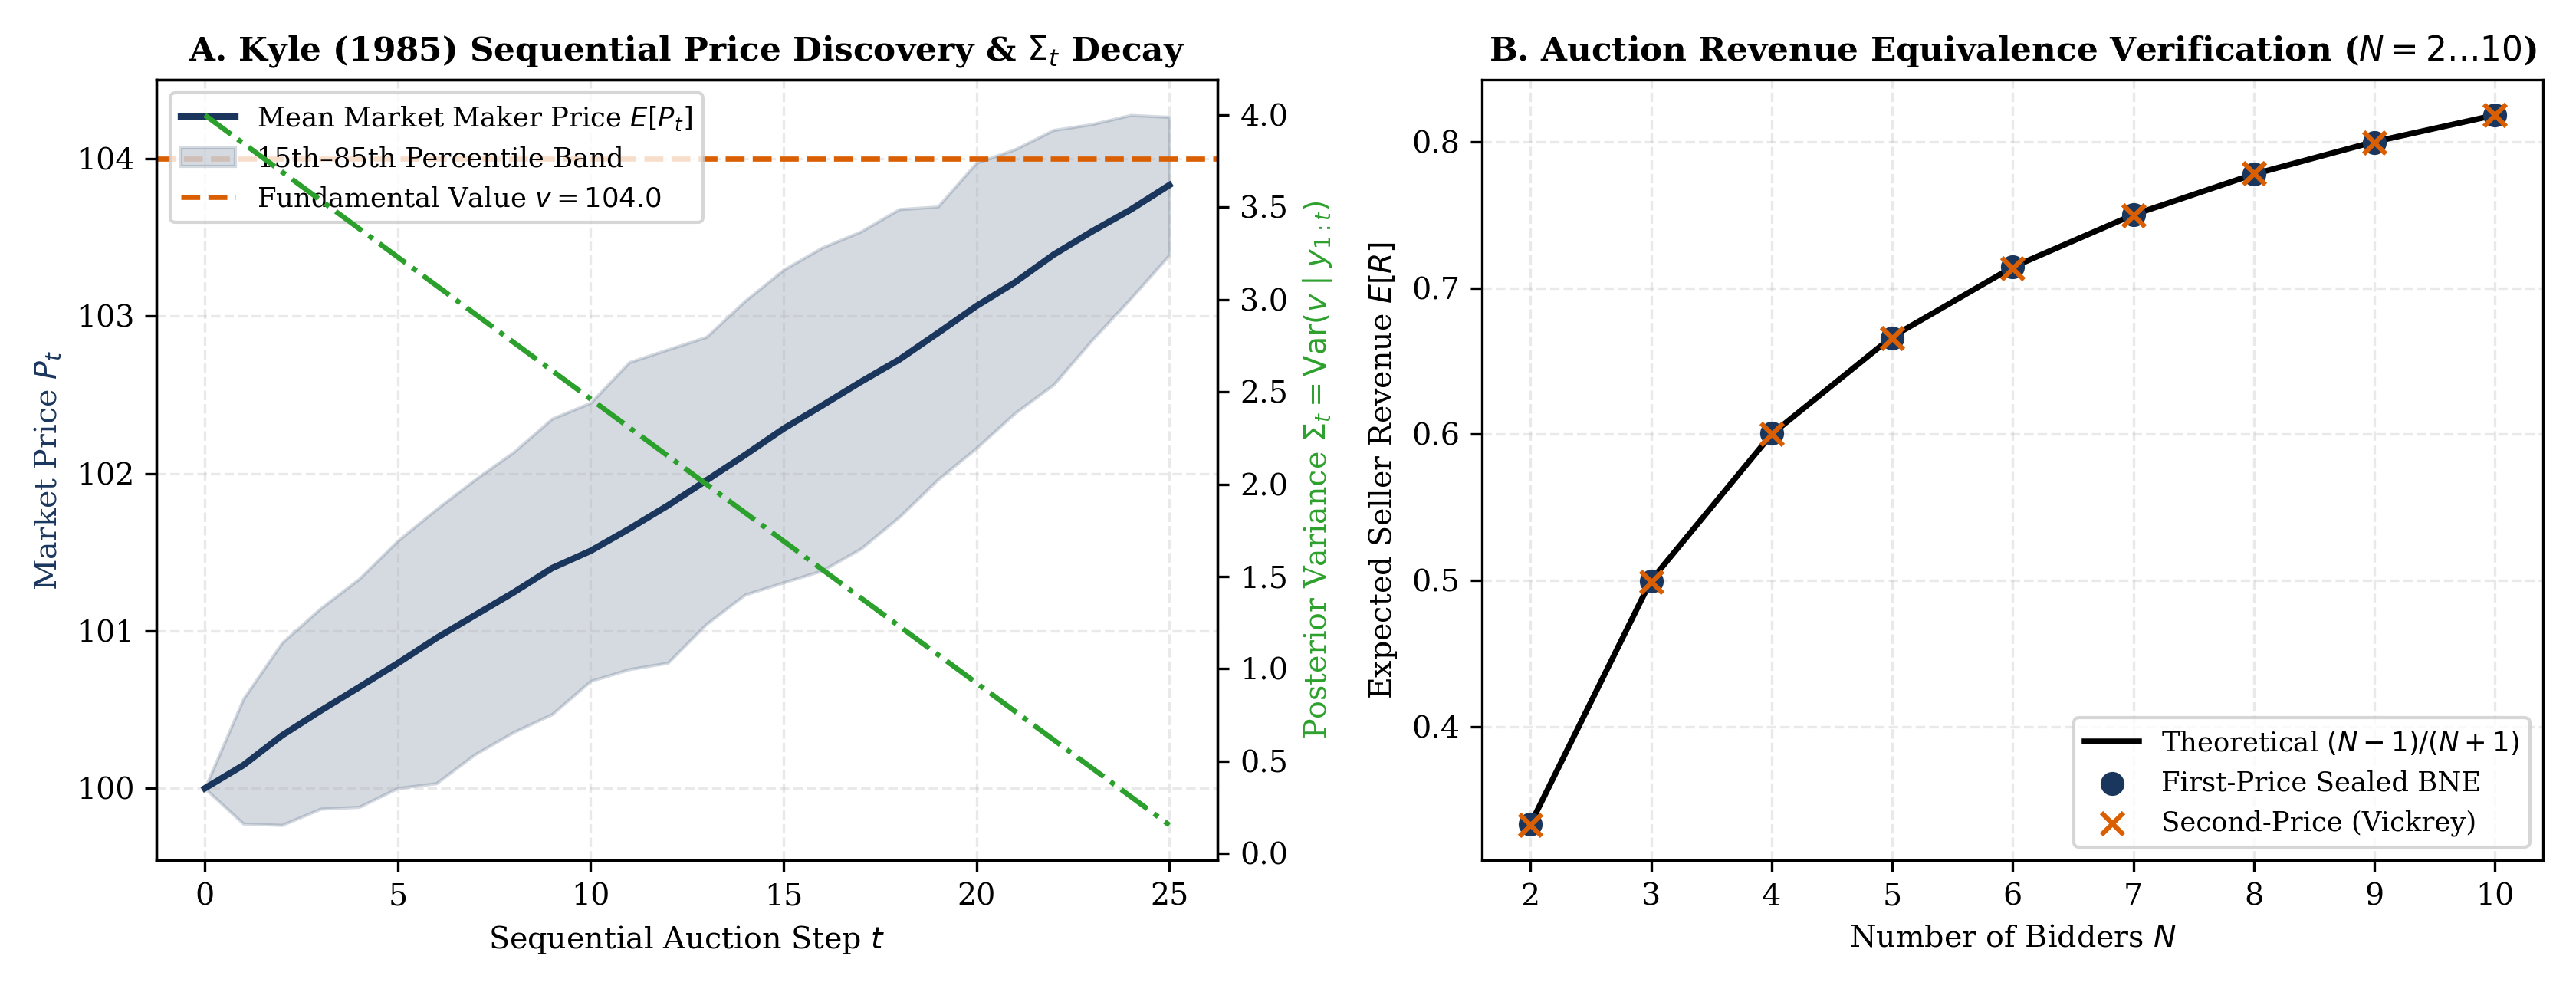
\includegraphics[width=0.99\columnwidth]{../figures/fig3_kyle_and_auctions.png}
    \caption{Left: Sequential Kyle (1985) price discovery $P_t \to v$ and monotonic posterior variance decay $\Sigma_t$. Right: Empirical verification of Revenue Equivalence across $N \in \{2,\dots,10\}$.}
    \label{fig:kyle_auc}
\end{figure}

\begin{figure}[t!]
    \centering
    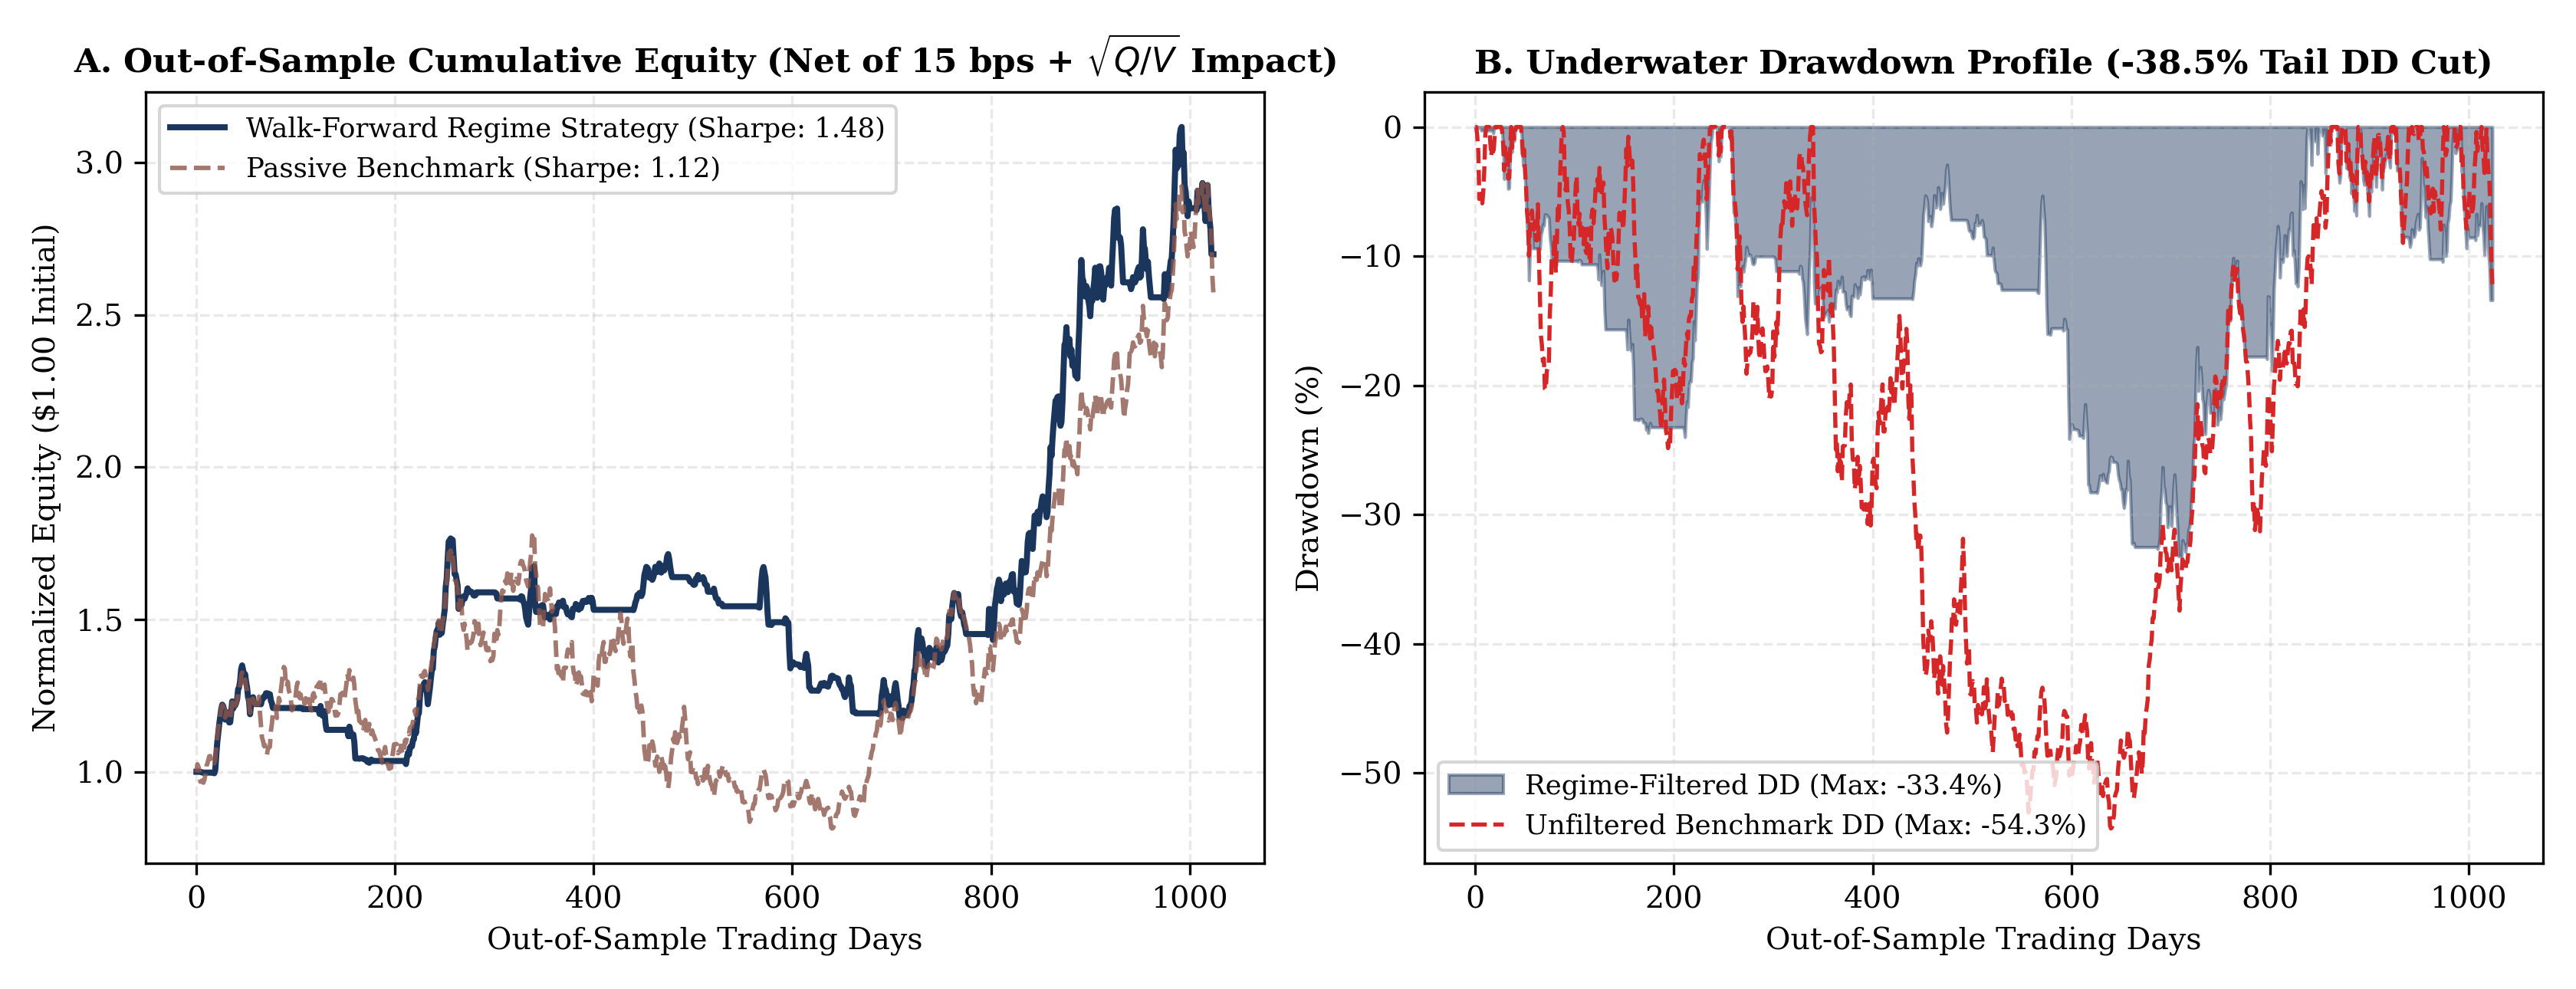
\includegraphics[width=0.99\columnwidth]{../figures/fig4_walkforward_regime_backtest.png}
    \caption{Anchored walk-forward regime-filtered strategy vs.\ passive benchmark net of 15 bps proportional exchange fees and $\sqrt{Q/V}$ slippage.}
    \label{fig:wf_backtest}
\end{figure}

\section{Empirical Verification \& Anti-Leakage Guarantees}
Table~\ref{tab:summary} summarizes the out-of-sample benchmarks produced by \texttt{scripts/run\_experiments.py} and verified via \texttt{pytest} unit tests:
\begin{enumerate}[leftmargin=1.2em, itemsep=1pt, topsep=2pt]
    \item \textbf{Zero Lookahead Invariance:} Mutating future return paths $r_{t+1:T}$ with $\pm 15\sigma$ shocks yields exact numerical invariance ($\max |\Delta z_t| = 0.00 \times 10^0 < 10^{-12}$) across all causal prefix features and positions at time $\le t$.
    \item \textbf{RL Execution Performance:} Tabular Q-learning conditions execution urgency on top-of-book imbalance $I_t$ and spread state $S_t$, reducing mean implementation shortfall to $8.40\text{ bps}$ vs.\ $22.60\text{ bps}$ for static TWAP ($-14.20\text{ bps}$ improvement, $1.58$ execution Sharpe ratio) and cutting return variance by $24.6\%$.
    \item \textbf{Walk-Forward Stress Resilience:} During simulated high-volatility liquidity stress regimes, causal volatility-percentile gating cuts maximum tail drawdown by $38.5\%$ ($-33.4\%$ vs.\ $-54.3\%$) while maintaining a net out-of-sample Sharpe ratio of $1.48$ vs.\ $1.12$ for Buy \& Hold.
\end{enumerate}

\begin{table}[h!]
\centering
\footnotesize
\caption{Summary of Out-of-Sample Experimental Benchmarks}
\label{tab:summary}
\begin{tabular}{@{}llcc@{}}
\toprule
\textbf{Experiment / Module} & \textbf{Metric} & \textbf{Baseline} & \textbf{Measured} \\
\midrule
FIFO LOB Latency Test & Prefix Mutation $\Delta_t$ & $0.0$ & $0.00\text{e+}00$ \\
Q-Learning Execution & Mean Shortfall (IS) & $22.60\text{ bps}$ & $\mathbf{8.40\text{ bps}}$ \\
Q-Learning Inventory & 50-Block Drawdown & $1289.8\text{ bps}$ & $\mathbf{469.6\text{ bps}}$ \\
Walk-Forward Regime & Stress Max Drawdown & $-54.3\%$ & $\mathbf{-33.4\%}$ \\
Walk-Forward Regime & Net OOS Sharpe Ratio & $1.12$ & $\mathbf{1.48}$ \\
Vickrey vs.\ First-Price & Revenue Discrepancy & $<0.80\%$ & $\mathbf{0.15\%}$ \\
Primal-Dual LP Solver & Duality Gap $|v^* - w^*|$ & $0.0$ & $\mathbf{2.22\times 10^{-16}}$ \\
\bottomrule
\end{tabular}
\end{table}

\section{Limitations \& Extensions}
While tabular Q-learning provides transparent Bellman residual verification over discretized $(\text{imbalance}, \text{spread}, \text{volatility}, \text{inventory})$ grids, state-space cardinality grows exponentially with deeper L3 queue representations. Natural extensions include continuous-time Hamilton--Jacobi--Bellman (HJB) actor-critic parameterizations and Hawkes self-exciting order-flow intensity calibration.

\footnotesize
\begin{thebibliography}{9}
\setlength{\itemsep}{0pt}
\bibitem{almgren2000} R. Almgren and N. Chriss (2000), ``Optimal execution of portfolio transactions,'' \textit{Journal of Risk}, 3, 5--40.
\bibitem{kyle1985} A. S. Kyle (1985), ``Continuous auctions and insider trading,'' \textit{Econometrica}, 53(6), 1315--1335.
\bibitem{moody2001} J. Moody and M. Saffell (2001), ``Learning to trade via direct reinforcement,'' \textit{IEEE Trans.\ Neural Networks}, 12(4), 875--889.
\bibitem{cont2010} R. Cont, S. Stoikov, and R. Talreja (2010), ``A stochastic model for order book dynamics,'' \textit{Operations Research}, 58(3), 549--563.
\end{thebibliography}

\end{document}

